\section{Convolutional Autoencoder}

To test the hypothesis that classification can be improved by using unsupervised methods to estimate the data distribution is investigated by using a convolutional autoencoder trained end-to-end on the data distribution, and then using the latent representation as input to a logistic regression classifier on the subset of data that has labels. This pipeline is outlined in section \ref{sec:architectures}, and the data are described in section \ref{sec:data}. The convolutional autoencoder has three configurations that we report results from. 
\begin{enumerate}[start=0, label={(\bfseries Ar\arabic*):}, ref={(Ar\arabic*)}]
	\item \label{item:clf_no_vgg} End-to-end training on data using kernel and filter architectures in a naive manner with decreasing kernel sizes, increasing filter sizes and a mirrored encoder-decoder structure
	\item \label{item:clf_freeze_vgg} Using the VGG16 network to compute a representation of the data which is compressed by one or more dense layers and finally reconstructed to the original image by a naively constructed decoder. 
	\item  \label{item:clf_tuning_vgg} Using the VGG16 network as the encoder, adjusting it's weights by the reconstruction loss with a naively constructed decoder. 
\end{enumerate}

\noindent Choosing an architecture for the convolutional autoencoder is the principal challenge to solve. We want to estimate if the reconstruction and optional latent losses relate to the classification accuracy achieved by the logistic regression classifier. \todo{add plot with reconst/loss vs f1 scores}

To aid in the understanding of the choice of architecture we compare the similarities between the optimal architectures for each of the data-sets. In the event that one dataset finds a configuration of lesser complexity that was not present in the others a verification run was computed with that configuration to ensure the validity of the performance measurement. \todo{add architecture tables, note on latent divergence?}


\begin{table}
\centering
\setlength{\extrarowheight}{15pt}
\hspace*{-0.5in}
\begin{tabular}{llll}
\toprule
Hyperparameter & \multicolumn{3}{c}{Value} \\
& Simulated & Filtered & Full \\
\midrule
\multicolumn{4}{l}{Convolutional parameters: } \\
\midrule
Number of layers & 3 & 6 & 6\\
Kernels & $[17, 15, 3]$ & $[9, 7, 5, 5, 5, 3]$ & $[11, 11, 11, 11, 5, 3]$ \\
Strides & $2$ & $2$ & $2$ \\
Filters & $[2, 16, 64]$ & $[8, 4, 16, 16, 16, 16]$ & $[16, 16, 16, 16, 32, 32]$ \\ 
\midrule
\multicolumn{4}{l}{Network parameters: } \\
\midrule
Activation & ReLU & LeakyReLU & LeakyReLU \\
Latent type & MMD & MMD & None \\
Latent dimension & $150$ & $50$ & $100$ \\
$\beta$ & \num{0.01} & $100$ & $ 100$  \\
\midrule
\multicolumn{4}{l}{Optimizer parameters: } \\
\midrule
$\eta$ &  \num{1e-5} & \num{0.0001} & \num{0.001} \\
$\beta_1$ & $0.73$ & $0.72$ & $0.25$ \\
$\beta_2$ & $0.99$ & $0.99$ & $0.99$ \\
\bottomrule
\end{tabular}
\caption{Hyperparameters that gives the strongest classifier performance on the three simulated, filtered and full datasets.}\label{tab:best_params_clf_convae}
\end{table}

For the best models found by random search we re-compute the performance with $K=5$ fold cross validation on the logistic regression classifier. We begin with the model using no information from the VGG16 benchmark, i.e. configuration \ref{item:clf_no_vgg}. It shows strong performance on the classification task for all datasets. The results are listed in table \ref{tab:clf_no_vgg}

\begin{table}
\centering
\subimport{plots/}{convae_clf_table}
\caption{Logistic regression classification $f1$ scores using the \ref{item:clf_no_vgg} architecture. The standard error is reported from a $K=5$ fold cross validation of the logistic regression classifier.}\label{tab:clf_no_vgg}
\end{table}

\noindent Furthermore we estimate the performance of the best models as a function of the number of labeled samples it sees. We select a random subsample from the labeled dataset and iteratively add to that dataset in increments of $n=100$ samples. This procedure is repeated a total of $N=10$ times to estimate the variability as a function of the selection process. The resulting runs are shown in figure \ref{fig:ac_n_labeled}

\begin{figure}
\centering
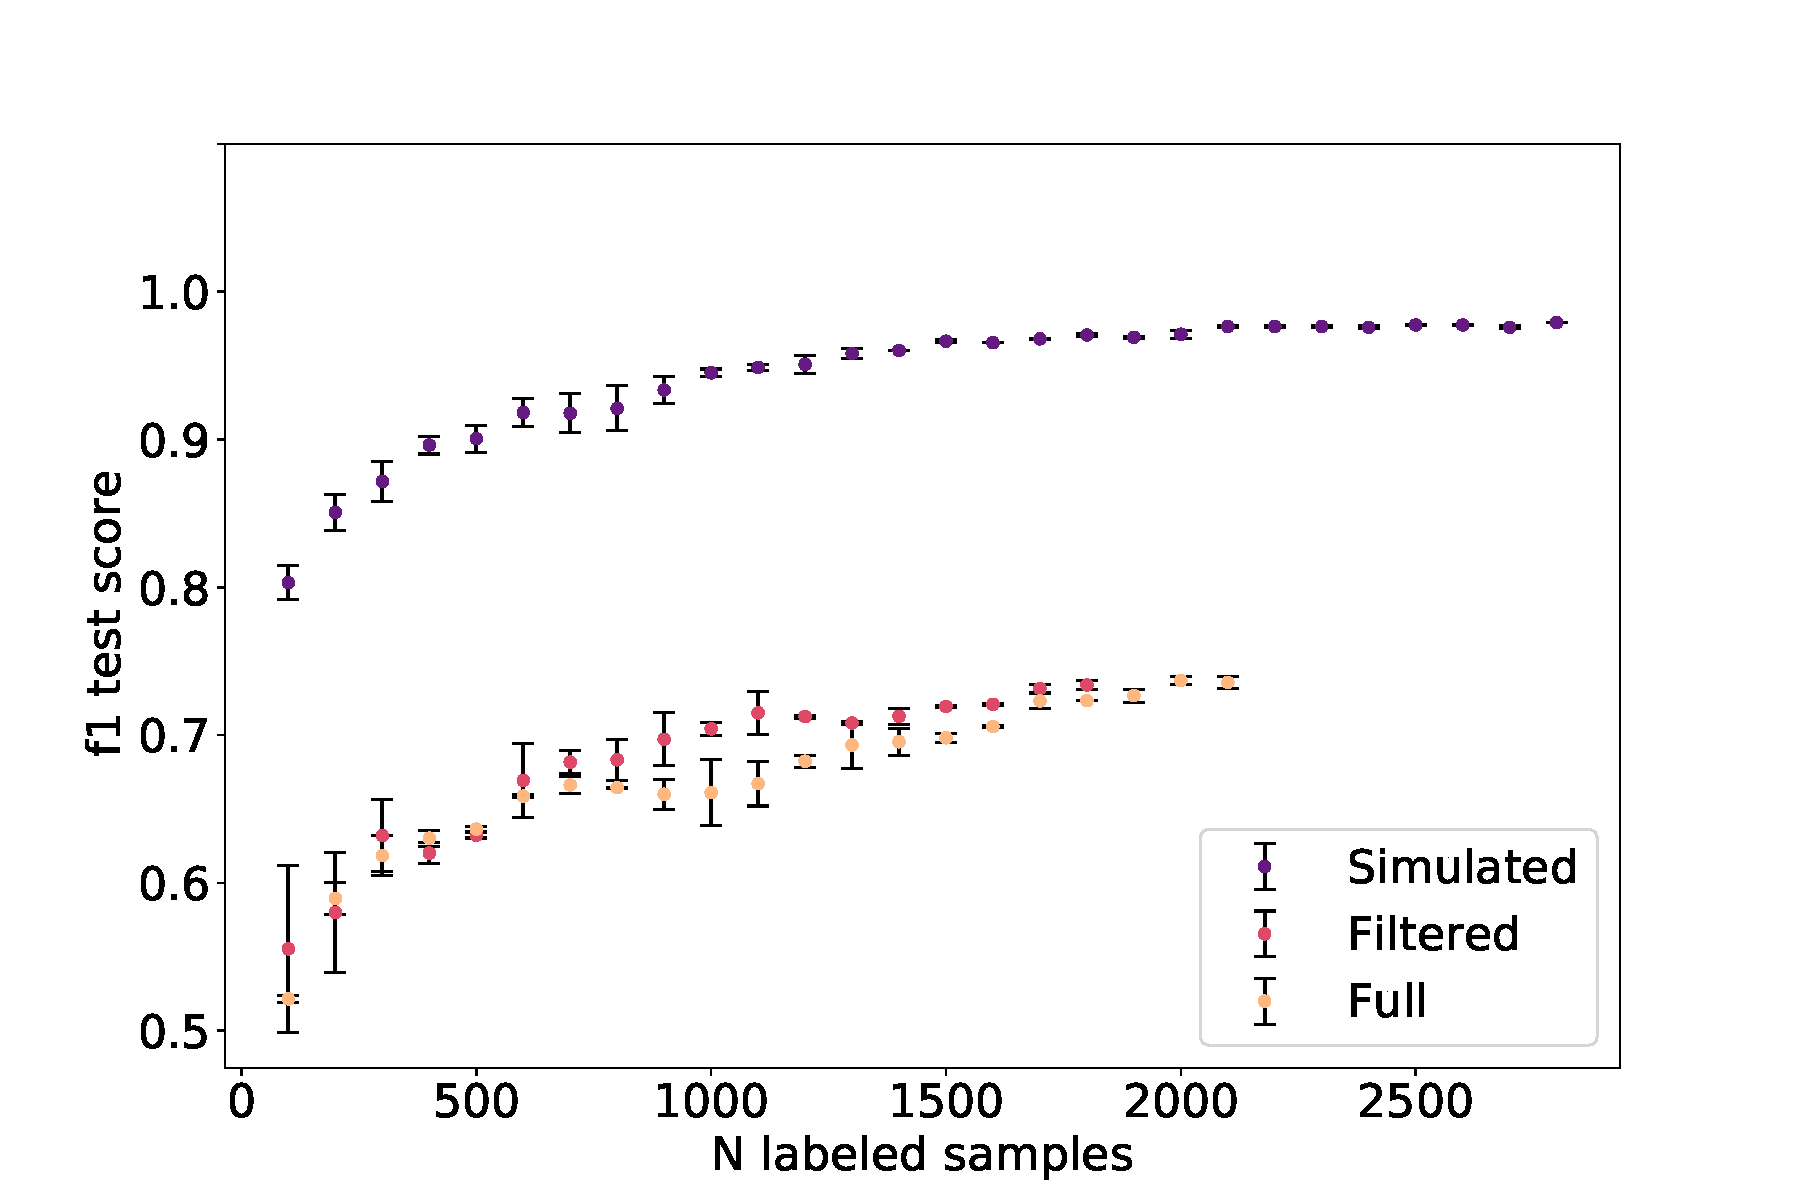
\includegraphics[width=\textwidth]{plots/ac_n_samples.pdf}
\caption[Autoencoder performance on labeled subsets]{Latent space classification performance with a logistic regression classifier on a \ref{item:clf_no_vgg} representation of each dataset. For each dataset a random subsample is drawn and iteratively added to in increments of $n=100$ data-points. To estimate the variance of this procedure we repeat the procedure $N=10$ times.}\label{fig:ac_n_labeled}
\end{figure}

\noindent Lastly we wish to qualitatively inspect the latent space with a 2D visualization of the latent space. We firstly process the latent space with a $D=50$ dimensional PCA and subsequently project to two dimensions with a t-SNE mapping of the data. This visualization is shown in figure \ref{fig:ac_tnse} and illustrates a good separation between the proton classes in general. 

\begin{figure}
\centering
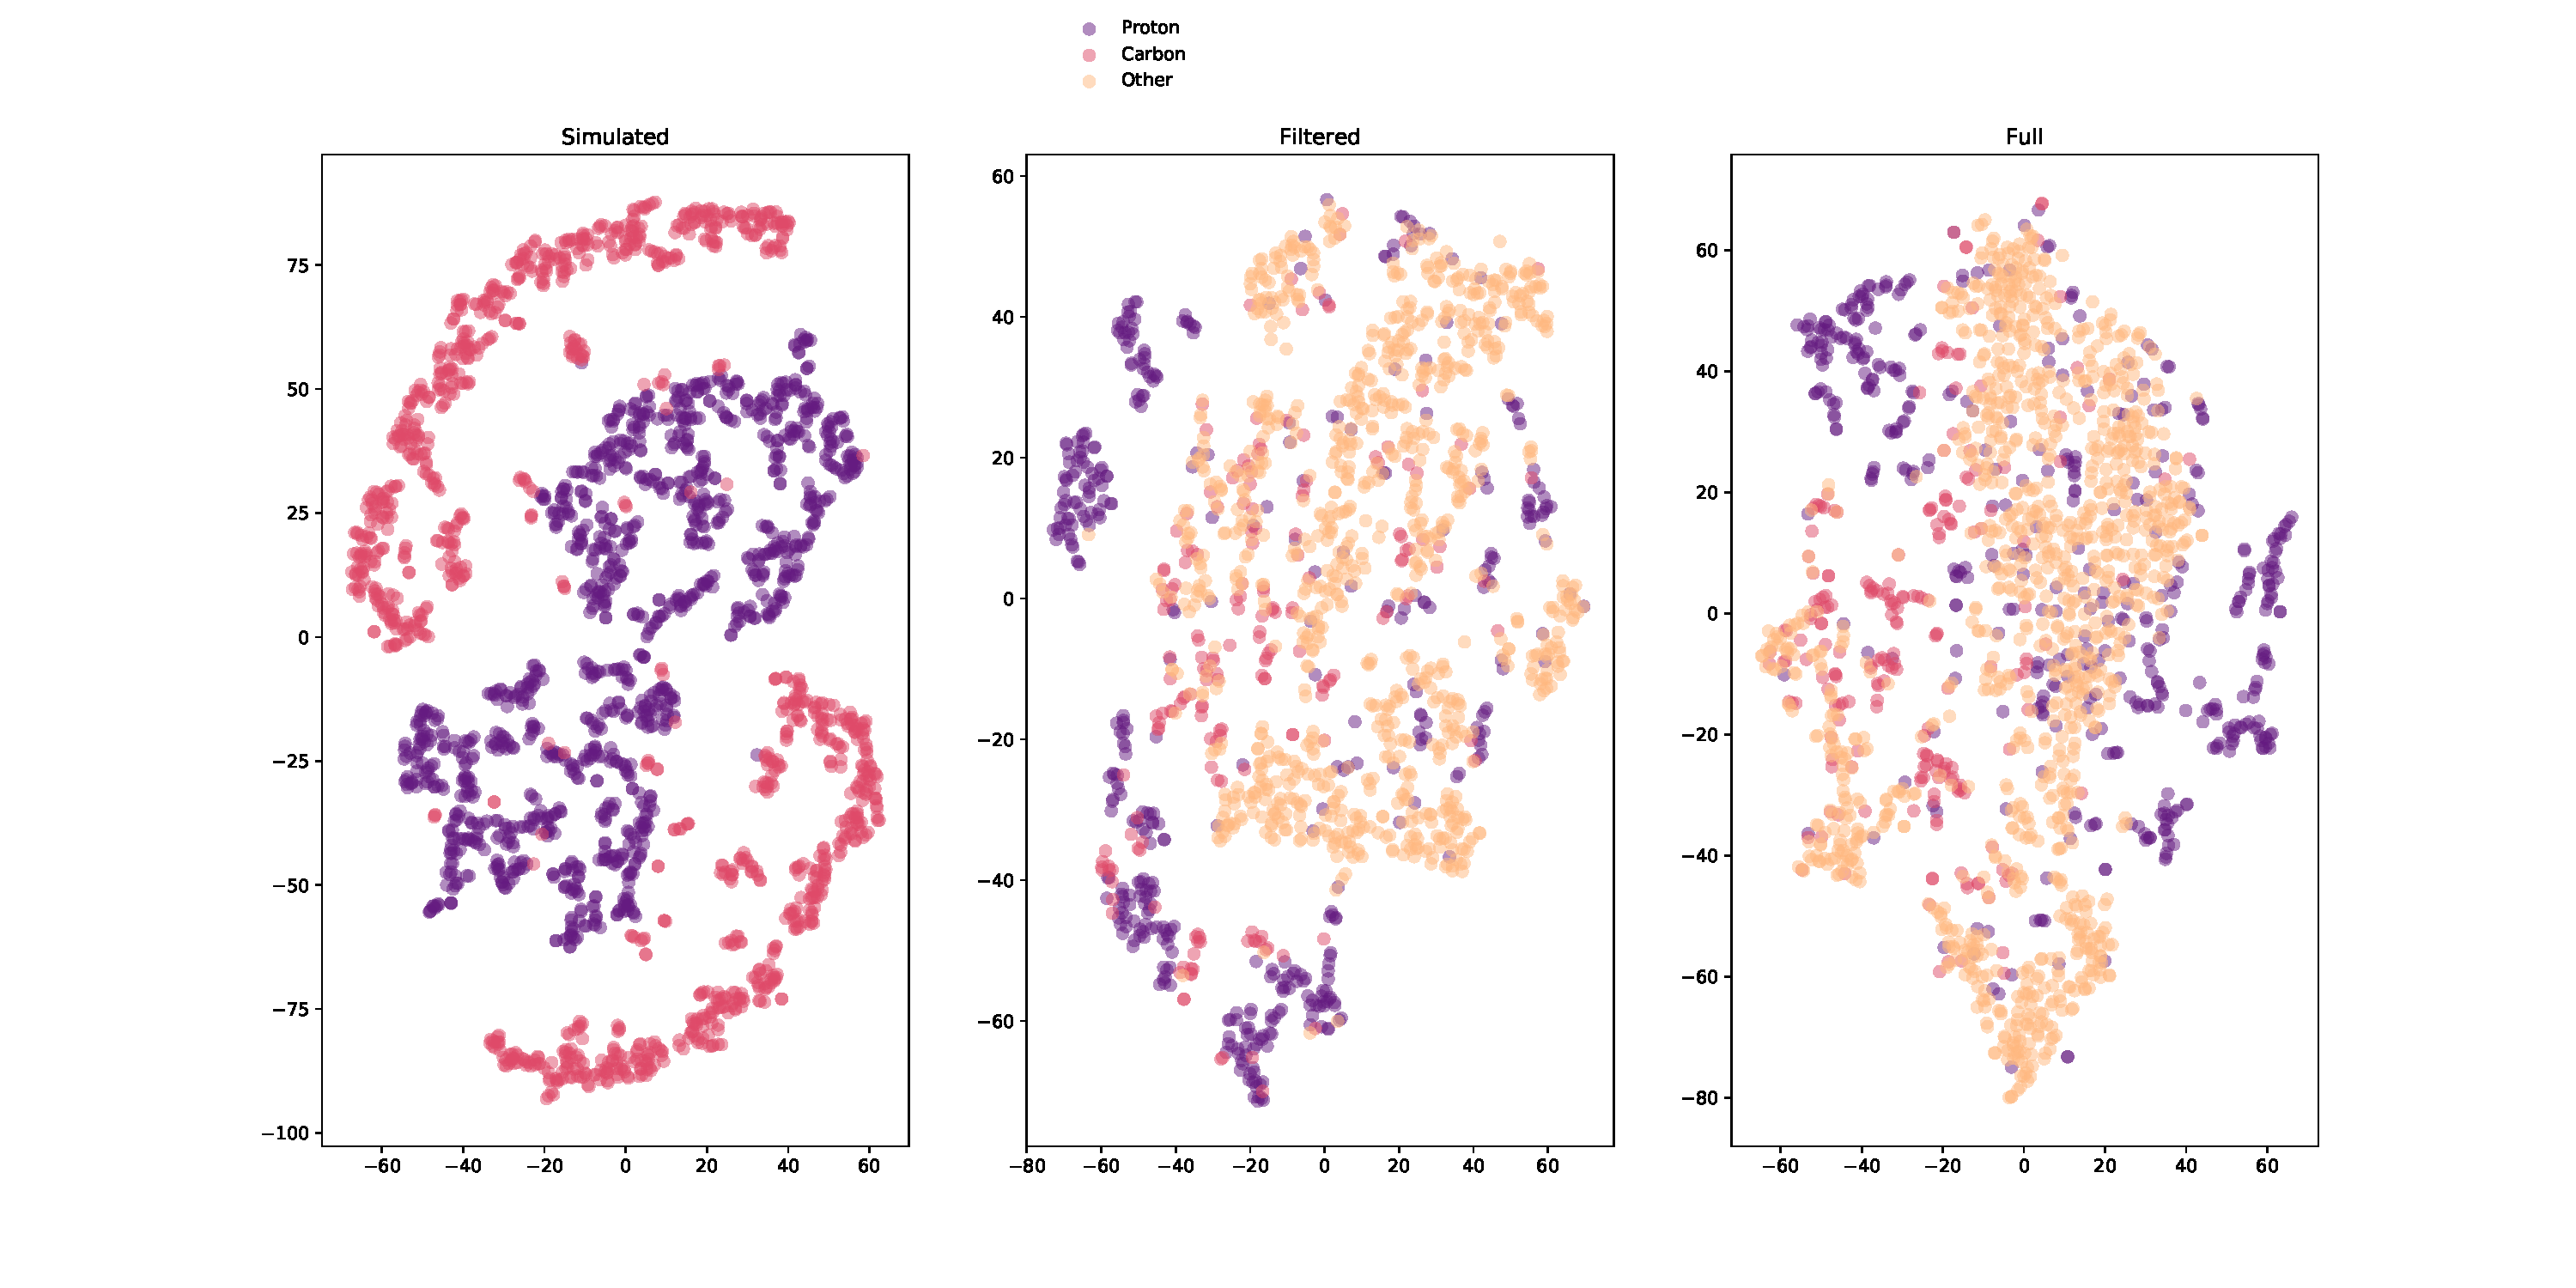
\includegraphics[width=\textwidth]{plots/ac_tsne.pdf}
\caption[autoencoder latent space visualization]{Visualizing the latent space of an \ref{item:clf_no_vgg} trained autoencoder. The mapping is a t-SNE projection of the latent space to two dimensions. We re-iterate that the axes have non-informative units.}\label{fig:ac_tnse}
\end{figure}

We repeat this process with using the VGG16 representation as initial input to the autoencoder model. This is configuration \ref{item:clf_freeze_vgg}. In the same manner as for the naive implementation we search over hyper-parameters, with the difference in the dense layer(s) included that transforms the VGG16 representation to the autoencoder latent space.

Each of the configurations found by the random search was then evaluated with $K=5$ fold cross validation to produce estimates of the $f1$ score, listed in table \ref{tab:clf_freeze_vgg}

\begin{table}
\centering
\subimport{plots/}{convae_vgg_clf_table}
\caption{Logistic regression classification $f1$ scores using the \ref{item:clf_freeze_vgg} architecture. The standard error is reported from a $K=5$ fold cross validation of the logistic regression classifier.}\label{tab:clf_freeze_vgg}
\end{table}

\noindent Furthermore we estimate the performance of the model as a function of the number of latent samples it is shown. In exactly the same manner as we did for the \ref{item:clf_no_vgg} architecture. The results of this search is shown in figure \ref{fig:vgg_ac_n_labeled}

\begin{figure}
\centering
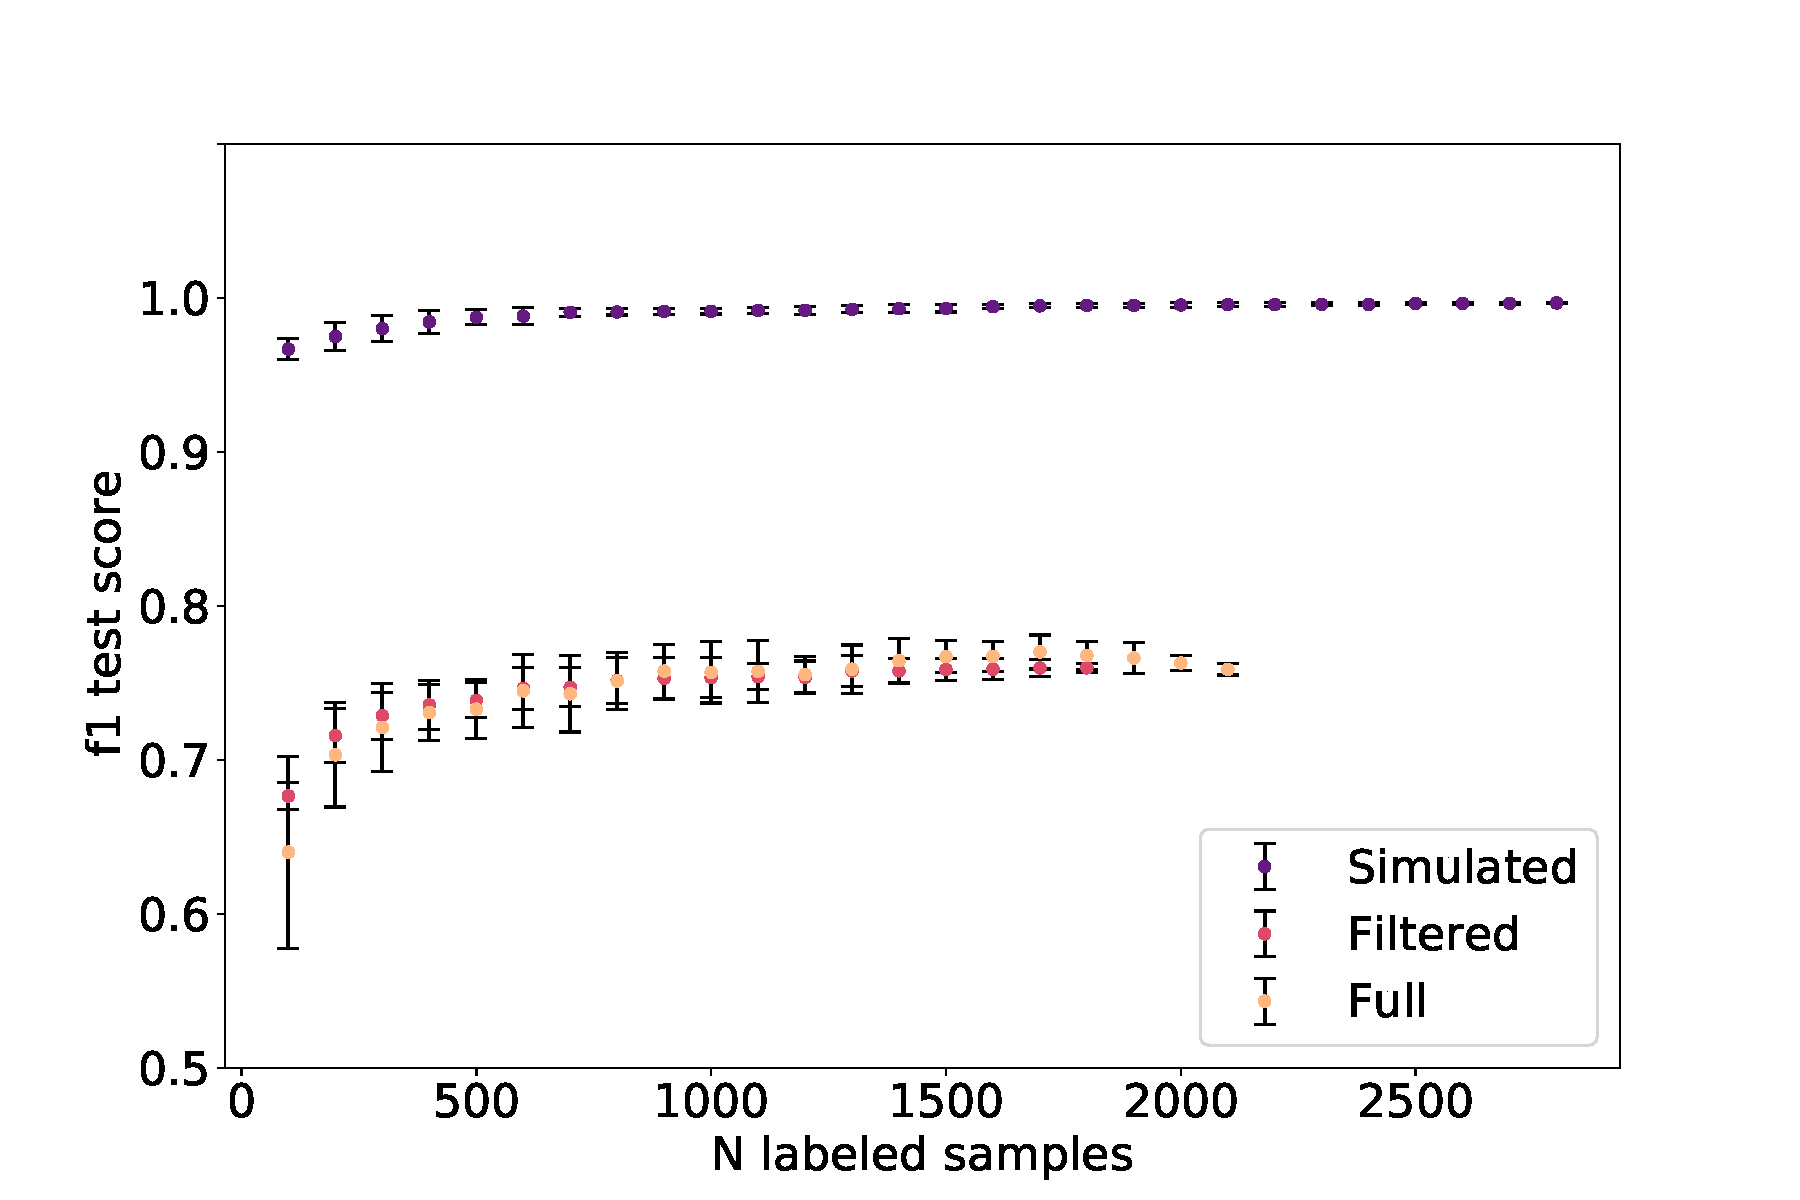
\includegraphics[width=\textwidth]{plots/vgg_ac_n_samples.pdf}
\caption[Autoencoder performance on labeled subsets]{Latent space classification performance with a logistic regression classifier on a \ref{item:clf_freeze_vgg} representation of each dataset. For each dataset a random subsample is drawn and iteratively added to in increments of $n=100$ data-points. To estimate the variance of this procedure we repeat the procedure $N=10$ times.}\label{fig:vgg_ac_n_labeled}
\end{figure}

Lastly for the architecture we project the latent space for comparison with the non-tuned VGG16 representation. 


\begin{figure}
\centering
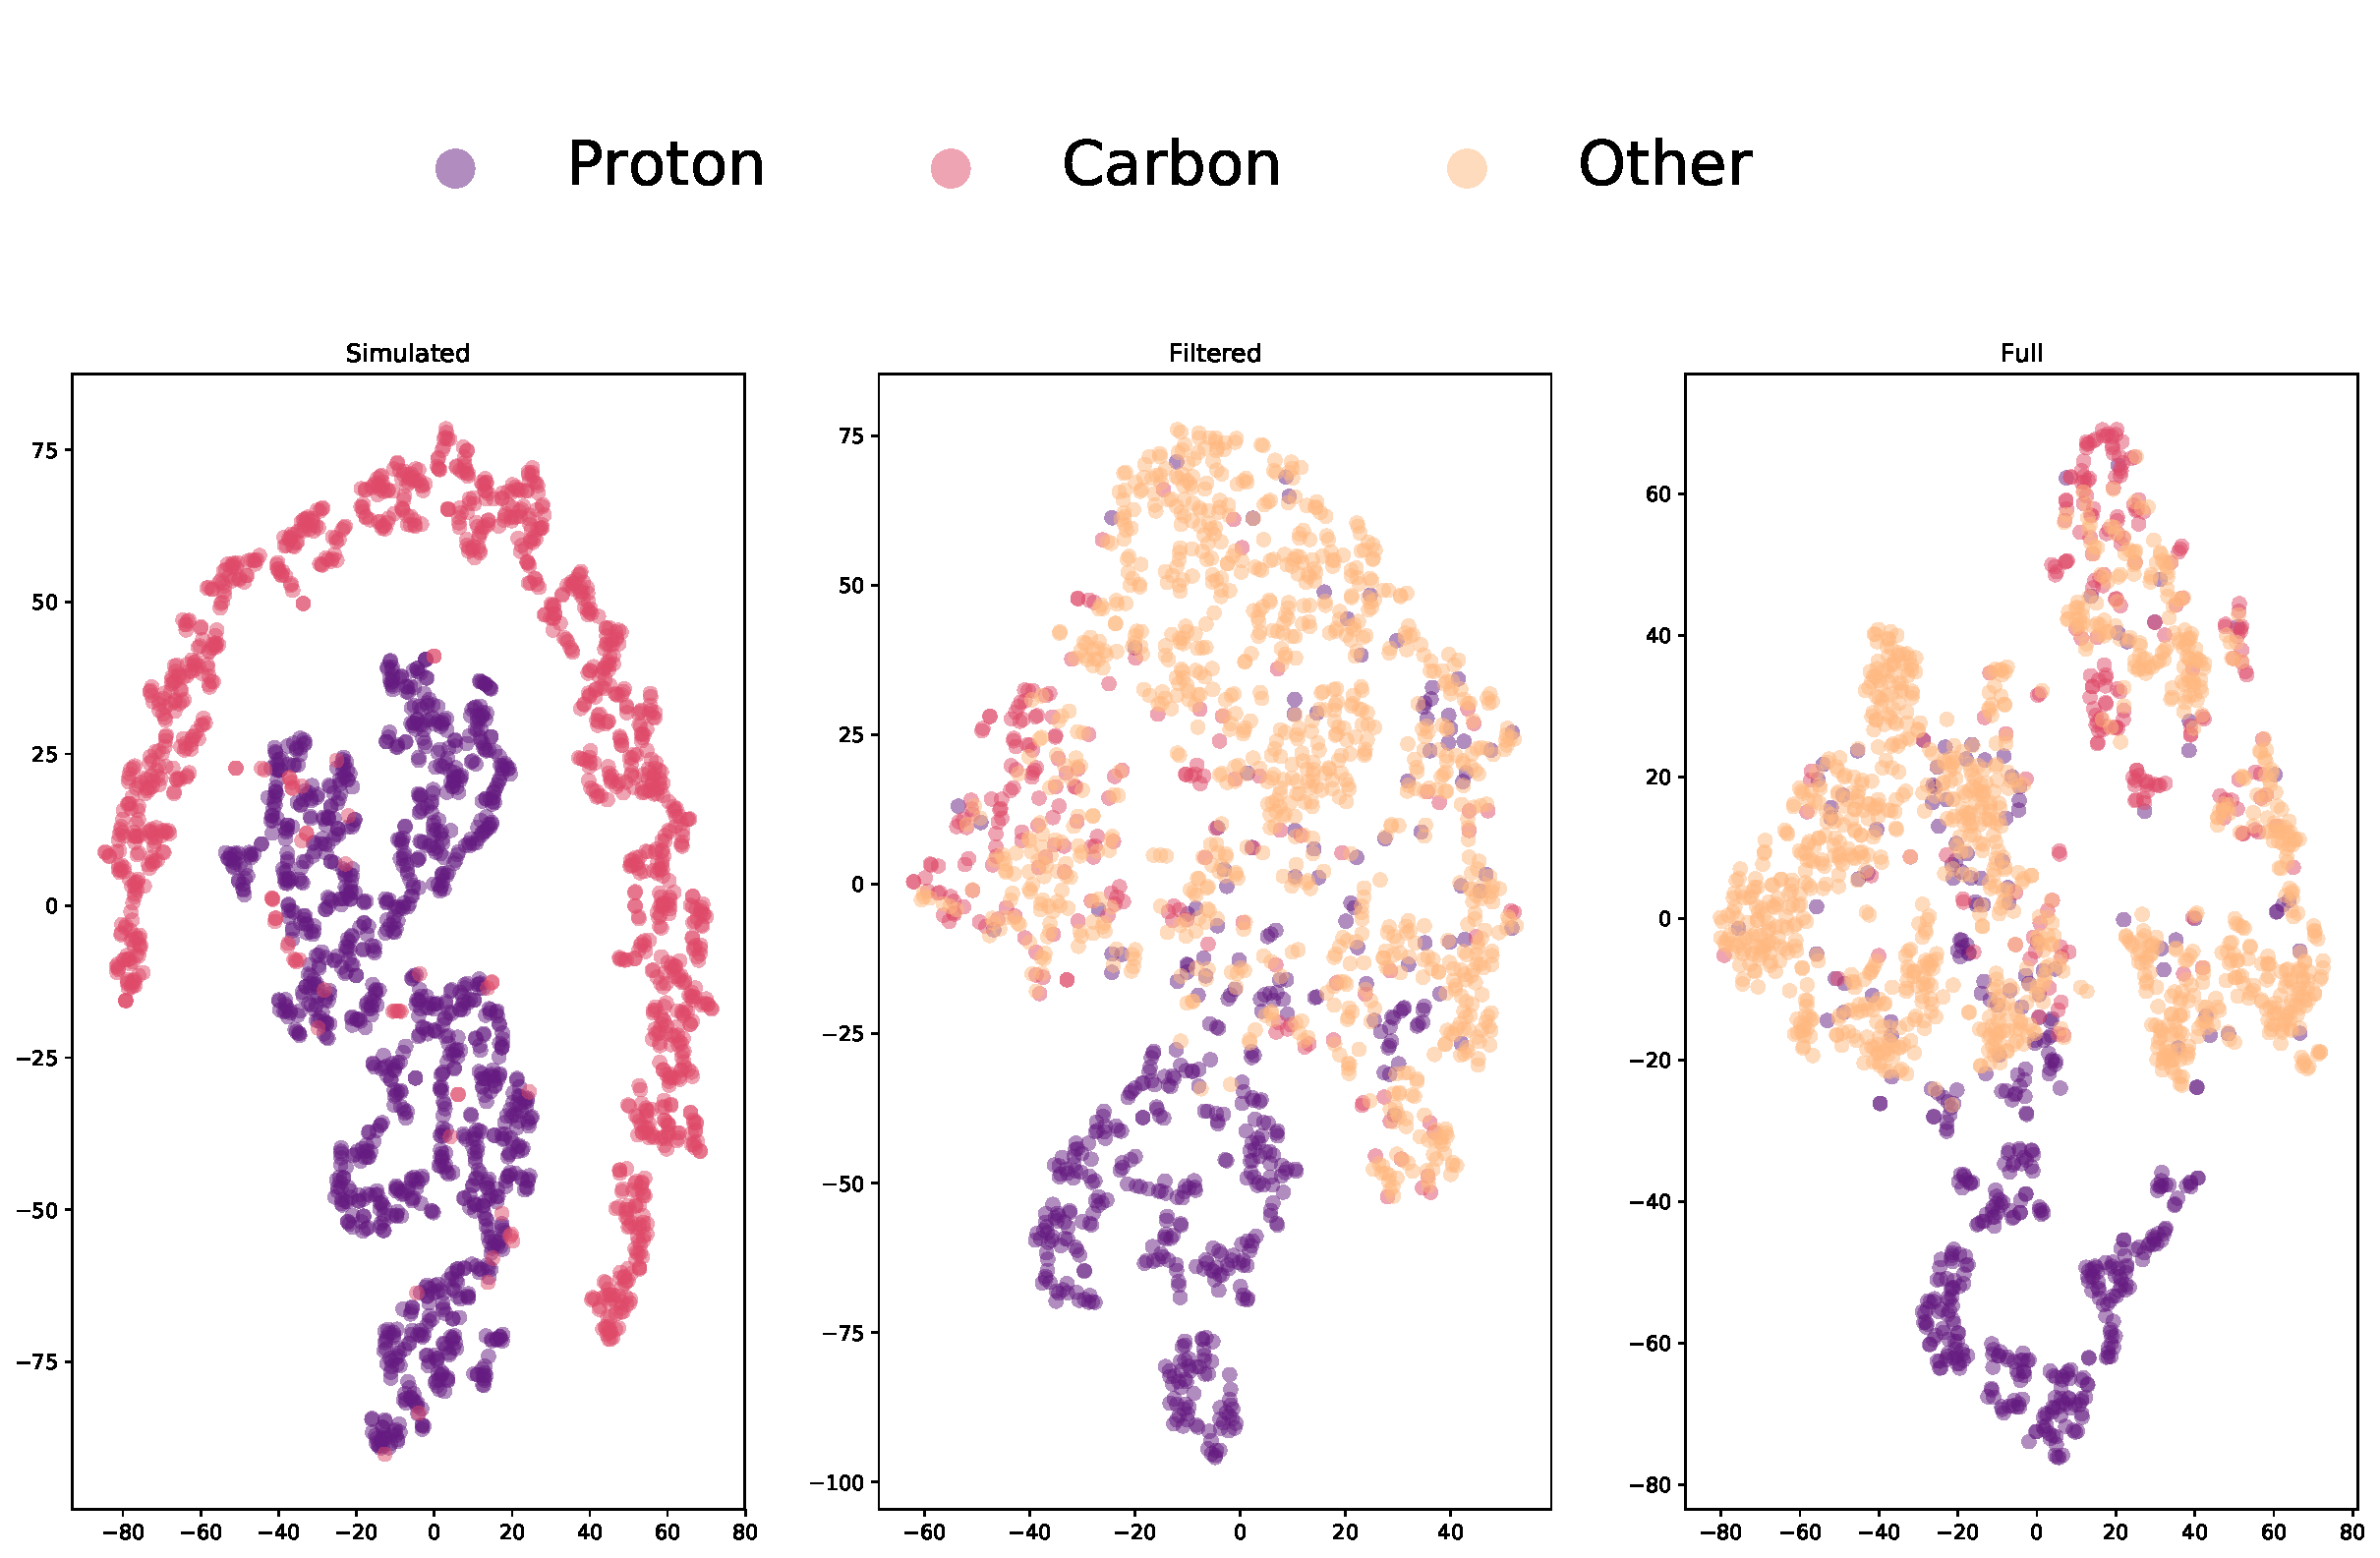
\includegraphics[width=\textwidth]{plots/vgg_ac_tsne.pdf}
\caption[VGG16-autoencoder latent space visualization]{Visualizing the latent space of an \ref{item:clf_freeze_vgg} trained autoencoder. The mapping is a t-SNE projection of the latent space to two dimensions.}\label{fig:ac_tnse}
\end{figure}
